% !TEX root = ./main.tex
% Garbage Collection
% ======================================================
\par \noindent 不可判定问题,使用可达性作为近似。
使用有向图,节点为程序变量和堆分配的记录,边为指针。
有向图的根节点是程序变量(寄存器、堆栈上的局部变量/形参、全局变量)。

\par \noindent \textbf{Mark-Sweep} Mark:从根节点出发遍历所有可到达的节点;Sweep:线性扫描扫描整个堆,将未标记的节点放入 free list。
垃圾回收后,程序恢复执行;每当在堆上分配新记录时,从 freelist 中获取一条记录;当 freelist 为空时,再次执行垃圾回收。
假设 $H$ 为堆大小,$R$ 可达数据数,一次 GC 的总时间 $c_1 R + c_2 H$,摊还时间为 $\frac{c_1 R + c_2 H}{H - R}$。
优化:显式栈:减少 DFS 递归调用的内存开销;指针反转:访问子节点时反转指针,以便回溯。
% 指针反转的具体算法不考
\par \noindent 优点:
1. 垃圾不多时效率高;
2.能够处理循环引用;
3. 对象/记录在 GC 期间不会移动。
缺点:
1. 垃圾多时效率低;
2. GC 时必须暂停程序执行;
3. 导致堆中的碎片化(这会导致缓存未命中、页抖动、更复杂的内存分配)。

\par \noindent \textbf{Reference Counting} 跟踪指向每个对象的指针数量(引用计数);每当建立新引用时,递增引用计数,反之递减;
当引用计数变为 0 时,对象是无法访问的垃圾。
优点:
1. GC 与程序执行交错,是 incremental overhead,没有 stop-and-collect 效应;
2. 相对容易实现;
3. 可与手动内存管理共存;
4. Spatial locality of reference is good(Access pattern to virtual memory pages no worse than the program, so no excessive paging);
5. 可以立即重用释放的单元。
缺点:
1. 无法处理循环引用;
2. 每次引用计数变化都需要更新计数器,开销大。

\par \noindent \textbf{Copying} 使用两个堆:from-space 和 to-space。当 from-space 耗尽时,遍历 from-space,将所有可达节点复制到 to-space;当下一次耗尽时,反转。
Pointer Forwarding:找到一个可达的记录时,将其复制到 to-space,并在 from-space 中存储指向新副本的转发指针。
\par \noindent Cheney’s Algorithm:将 to-space 划分为三个连续区域,使用 BFS 遍历可达数据,从 from-space 复制到 to-space。

\begin{figure}[H]
    \centering
    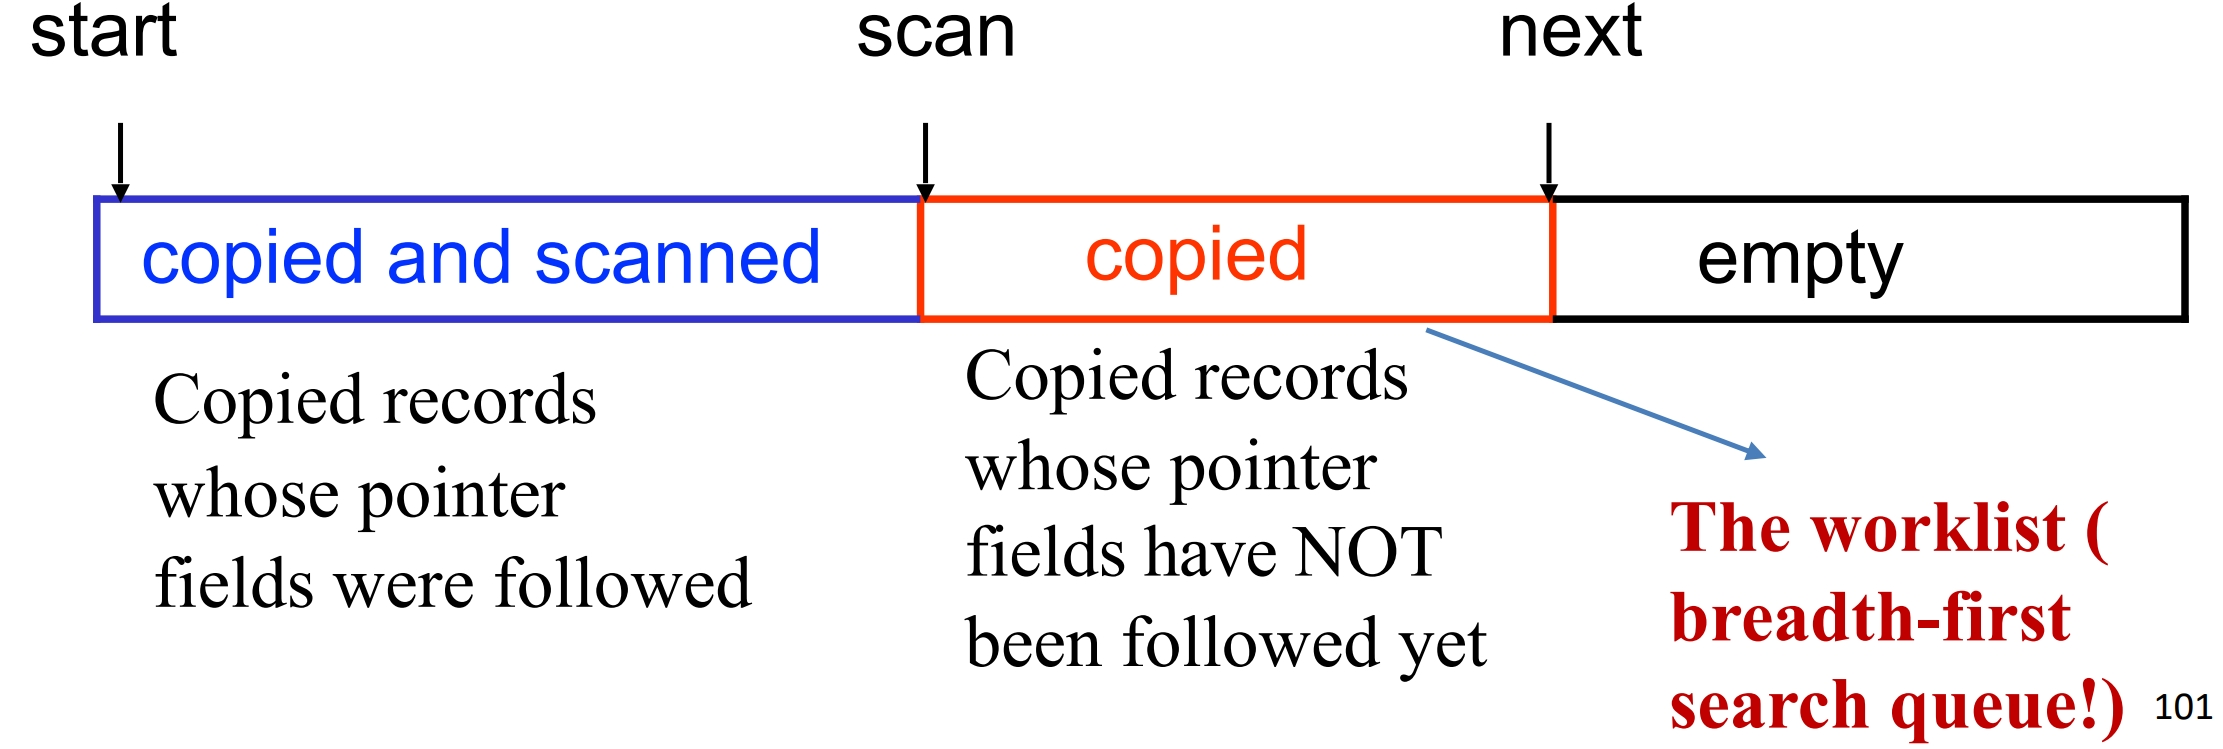
\includegraphics[width=0.8\linewidth]{figures/gc1.png}
\end{figure}

\begin{figure}[H]
    \centering
    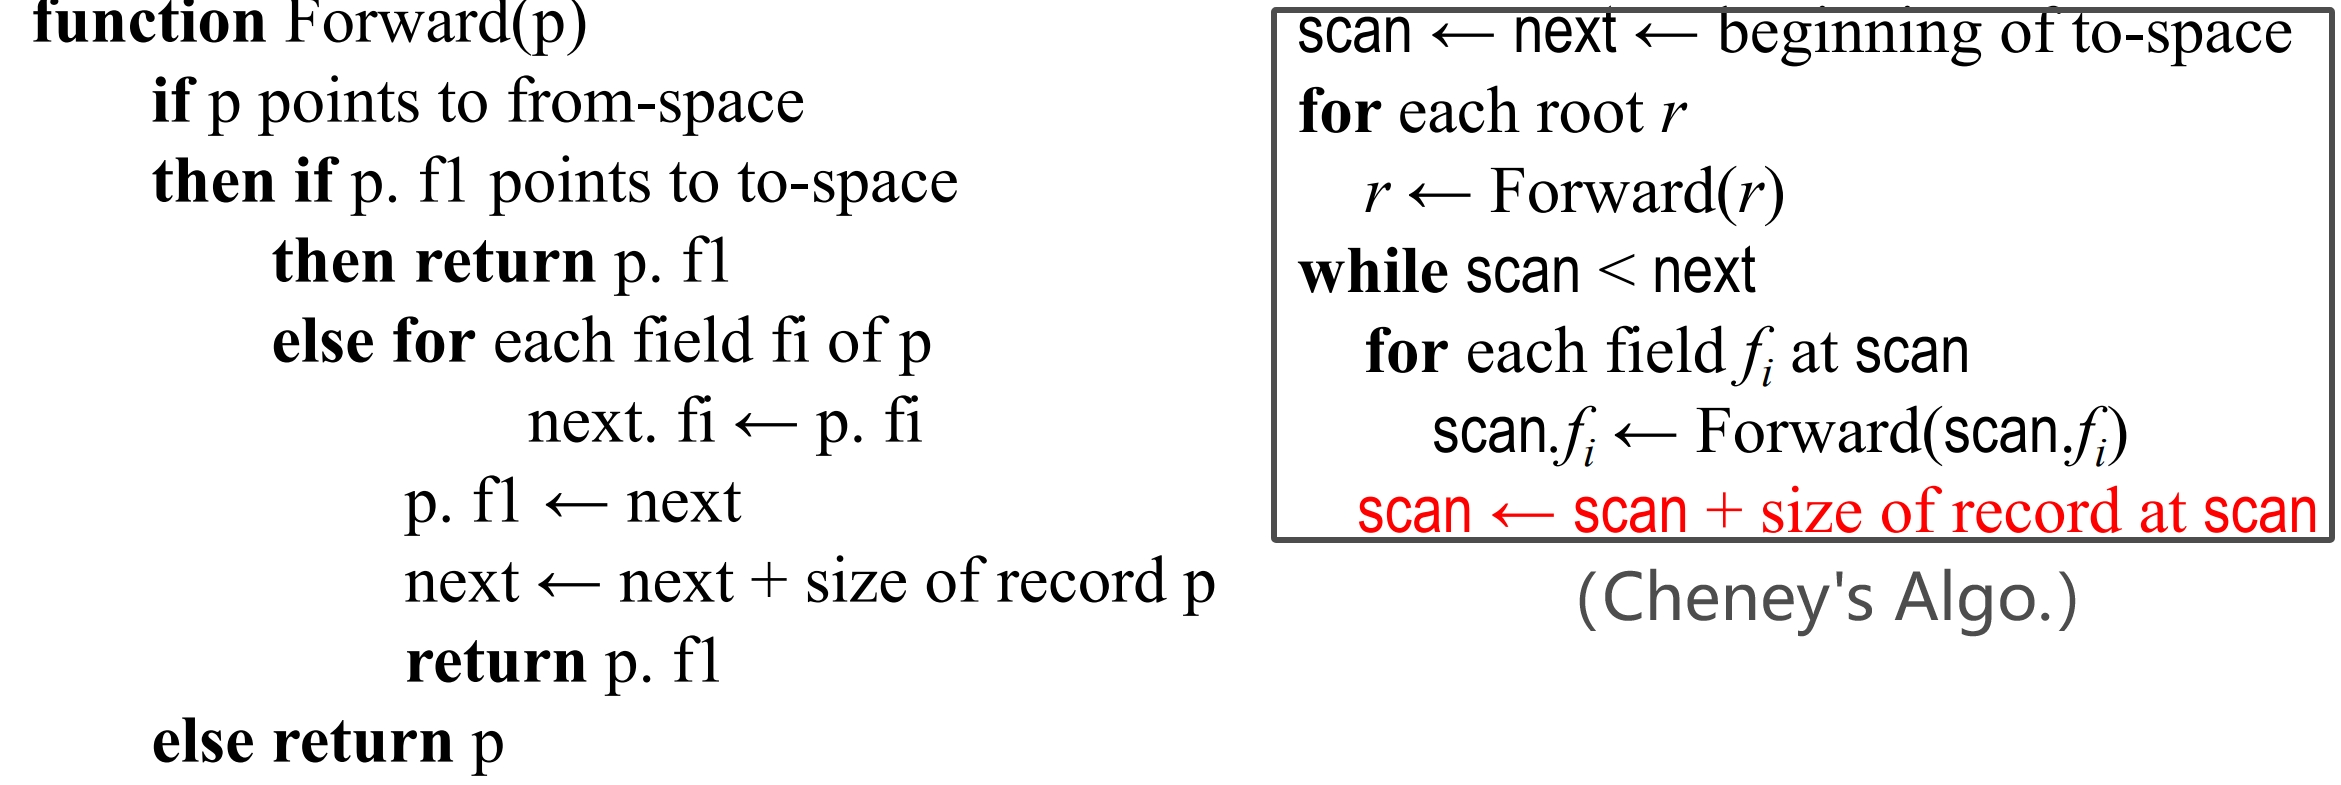
\includegraphics[width=0.8\linewidth]{figures/gc2.png}
\end{figure}

\par \noindent 改进 BFS 带来的局部性差的问题:使用 BFS,但是每当复制对象时,查看是否可以在它附近复制一些子项。

\par \noindent 优点:
1. 简单,无需栈或指针反转;
2. 运行时间与活跃的对象数量成正比;
3. 空闲空间连续;
4. 自动压缩消除碎片化;
5. 是许多后续算法的基础。
缺点:
1. 一半内存被浪费;
2. 局部性差(Cheney’s Algorithm);
3. 需要精确的类型信息(指针或非指针)。

\par \noindent 编译器需要为 GC :
1. Generating code that allocate records;
2. Describing locations of roots for each garbage collection cycle;
3. Describing the layout of data records on the heap;
4. Generating instructions to implement a read or write barrier(for some versions of incremental collection);
5. \dots

\par \noindent \textbf{Fast Allocation (for Copying Collection)} 
分配记录的过程:
1. Call the allocate function;
2. Test next + N < limit ? (If the test fails, call GC);
3. Move next to result;
4. Clear M[next], M[next+1], ..., M[next + N - 1];
5. next <- next + N;
6. Return from the allocate function。
这里的步骤 2 和 5 无法消除,通过在寄存器中保留 next 和 limit,步骤 2 和 5 总共可以在 3 条指令中完成,
分配记录的成本可以降低到大约 4 条指令,然后进行 GC。

\par \noindent Describing Data Layouts:类描述符生成,语义分析阶段。

\par \noindent Exact Root Description (Pointer Map),包含栈上的指针和 callee-saved 寄存器中的指针。
在何处插入 Pointer Map 取决于 GC 在何时触发:分配时:在 \texttt{alloc\_record}之前插入;递归调用时:插入所有函数调用。
To find all the roots, the collector starts at the top of the stack and scans downward.
1. Each return address keys the pointer-map entry that
describes the next frame;2.In each frame, the collector marks (or forwards, if copying collection) from the pointers in that frame.
Callee-save registers need special handling, the pointer map for g must describe 
which of its callee-save registers contain pointers at the call to h and which are “inherited” from f.

\par \noindent Derived Pointers:\texttt{t1 <- a - 2000; t2 <- t1 + i; t3 <- M[t2]},
We say that t1 is derived from the base pointer \texttt{a}. 
The pointer map must identify each derived pointer and tell its base pointer.
When the collector relocates \texttt{a} to address \texttt{a'}, it must adjust \texttt{t1} to point to address \texttt{t1 + a' - a},
\texttt{a} must remain live as long as \texttt{t1} is live.